\section{Comparison to State-of-the-art}

In this section we report on an experiment using both CLSmith and CLgen for 48 hours each.

Total runtime for a test cases consists of the generation time, the time to execute the test harness on a device, and, if required, the time to reduce the test case.

Like-for-like comparison of CLgen and CLSmith. Run the full stack of generation-execution-difftest-reduce for a fixed period of time, and report the number of bugs found. Is CLgen faster? Do we have to reject test cases?

\subsection{Testing Methodology}

Both testing frameworks were used for 48 hours each. CLSmith was configured with default settings. CLReduce was configured with the default settings (four parallel reduction threads).

\subsection{Results}

Table~\ref{tab:results}.

\begin{table*}
	\scriptsize %
	\centering %
	\begin{tabular}{lll | rrrrr | rrrrr }
  \toprule
  & & & \multicolumn{5}{c|}{\textbf{CLSmith}} & \multicolumn{5}{c}{\textbf{CLgen}} \\
  \textbf{\#.} & \textbf{Device} & $\pm$ &
  \textbf{w} & \textbf{bf} & \textbf{c} & \textbf{to} & \textbf{\% of total} &
  \textbf{w} & \textbf{bf} & \textbf{c} & \textbf{to} & \textbf{\% of total} \\
  \midrule
  \multirow{ 2}{*}{1} & \multirow{ 2}{*}{GeForce GTX 1080} & $-$ & 0 & 0 & 17 & 25 & 0.8\%       & 10 & 45 & 28 & 5 & 0.4\% \\& & $+$ & 5 & 0 & 63 & 15 & 1.5\% & 14 & 28 & 12 & 14 & 0.3\% \\
\hline
\multirow{ 2}{*}{2} & \multirow{ 2}{*}{GeForce GTX 780} & $-$ & 3 & 0 & 22 & 37 & 0.9\%       & 617 & 406 & 65 & 42 & 25.9\% \\& & $+$ & 0 & 0 & 10 & 37 & 0.7\% & 281 & 375 & 37 & 68 & 22.9\% \\
\hline
\multirow{ 2}{*}{3} & \multirow{ 2}{*}{Intel HD Haswell GT2} & $-$ & 0 & 0 & 0 & 0 & 0.0\%       & 108 & 473 & 20 & 0 & 1.2\% \\& & $+$ & 0 & 0 & 0 & 0 & 0.0\% & 22 & 39 & 6 & 0 & 0.2\% \\
\hline
\multirow{ 2}{*}{4} & \multirow{ 2}{*}{Intel E5-2620 v4} & $-$ & 0 & 563 & 192 & 0 & 11.2\%       & 3 & 10 & 93 & 1 & 0.3\% \\& & $+$ & 0 & 595 & 434 & 1 & 14.5\% & 1 & 7 & 110 & 3 & 0.3\% \\
\hline
\multirow{ 2}{*}{5} & \multirow{ 2}{*}{Intel E5-2650 v2} & $-$ & 0 & 0 & 0 & 0 & 0.0\%       & 2 & 65 & 131 & 1 & 23.9\% \\& & $+$ & 0 & 0 & 61 & 0 & 1.1\% & 8 & 66 & 138 & 3 & 25.1\% \\
\hline
\multirow{ 2}{*}{6} & \multirow{ 2}{*}{Intel i5-4570} & $-$ & 0 & 570 & 0 & 0 & 8.3\%       & 15 & 362 & 156 & 10 & 20.2\% \\& & $+$ & 0 & 629 & 0 & 0 & 8.2\% & 6 & 167 & 170 & 10 & 31.6\% \\
\hline
\multirow{ 2}{*}{7} & \multirow{ 2}{*}{Intel Xeon Phi} & $-$ & 6 & 0 & 131 & 5 & 2.8\%       & 19 & 30 & 0 & 73 & 0.9\% \\& & $+$ & 1 & 0 & 0 & 4 & 0.3\% & 12 & 32 & 0 & 65 & 0.8\% \\
\hline
\multirow{ 2}{*}{8} & \multirow{ 2}{*}{POCL (Intel E5-2620)} & $-$ & 0 & 0 & 56 & 2 & 0.9\%       & 2 & 6 & 850 & 7 & 2.8\% \\& & $+$ & 0 & 0 & 8 & 18 & 0.4\% & 1 & 7 & 930 & 1 & 2.9\% \\
\hline
\multirow{ 2}{*}{9} & \multirow{ 2}{*}{ComputeAorta (Intel E5-2620)} & $-$ & 0 & 0 & 0 & 11 & 0.2\%       & 15 & 620 & 85 & 0 & 38.8\% \\& & $+$ & 9 & 0 & 177 & 35 & 3.1\% & 19 & 563 & 49 & 6 & 39.4\% \\
\hline
\multirow{ 2}{*}{10} & \multirow{ 2}{*}{Oclgrind Simulator} & $-$ & 0 & 0 & 0 & 8 & 0.4\%       & 6 & 3 & 13 & 80 & 0.3\% \\& & $+$ & 0 & 0 & 0 & 14 & 0.7\% & 7 & 2 & 9 & 50 & 0.2\% \\
  \bottomrule
\end{tabular}


	\caption{Testing results using CLSmith and CLgen for 48 hours each. Configuration \#. as per Table~\ref{tab:platforms}. $\pm$ denotes optimizations off ($-$) vs on ($+$). The remaining columns denote wrong-code (w), build failure (\textbf{bf}), runtime crash (\textbf{c}), timeout (\textbf{to}), passed (\textbf{\cmark}), and rejected (\textbf{\xmark}) test cases for CLSmith and CLgen, respectively. \cc{Asterisk in 'total' column means the full 48 hours of data have not yet been collected. All results are excluding reductions.}}
	\label{tab:results}
\end{table*}

How long do reductions take? How many CLgen test cases can we run in that amount of time? Given the ratio of interesting CLgen test cases, how many more bugs could we find in the amount of time it takes to run a single reduction?

\subsection{Test Case Size}

Median CLSmith kernel is 1086 lines long (excluding headers, and using CLSmith \texttt{--short} option).

For ``interesting'' programs: median CLgen kernel size is 12 lines. Median reduced CLSmith kernel size is 43 lines (894 lines before reduction). Figure~\ref{fig:kernel-sizes}.

Potentially interesting questions: What is the total lines of code which get run on each device during the tests? CLgen programs are smaller, but we get through more of them.

\cc{CLgen test cases are two orders of magnitude smaller than CLSmith programs which have been reduced.}

\cc{What is the bug rate per line of code?}

\begin{figure}
	\centering %
	\includegraphics[width=\columnwidth]{build/img/runtimes}%
	\caption{%
		Runtimes, excluding timeouts.%
	}%
	\label{fig:runtimes} %
\end{figure}


\begin{figure}
	\centering %
	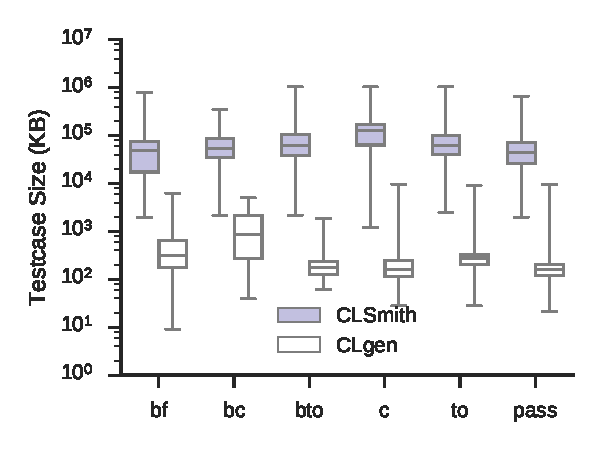
\includegraphics[width=\columnwidth]{build/img/kernel-sizes}%
	\caption{%
		Kernel line counts, grouped by classification. CLSmith programs with \emph{w} classification have been reduced.%
	}%
	\label{fig:kernel-sizes} %
\end{figure}


\begin{figure}
	\centering %
	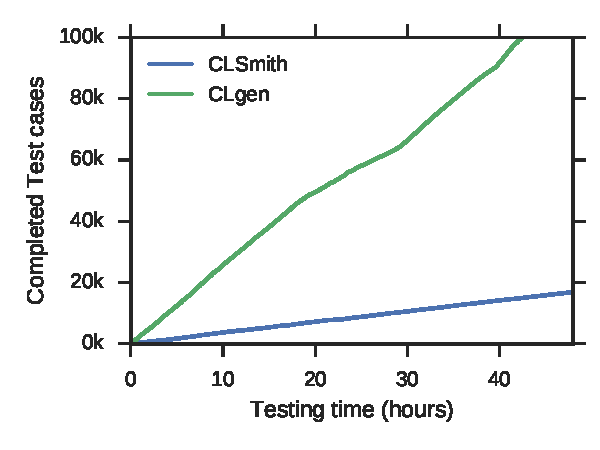
\includegraphics[width=\columnwidth]{build/img/total-tests}%
	\caption{%
		Test cases.%
	}%
	\label{fig:total-tests} %
\end{figure}